\documentclass{article}

% Import packages
\usepackage{amsmath}
\usepackage{listings}
\usepackage{graphicx}
\usepackage{float}
\usepackage{color}
\usepackage{booktabs}
\usepackage{caption}
\usepackage{hyperref}
\usepackage{placeins}

% Tweak vertical caption spacing
\captionsetup[table]{skip=10pt}

% Custom commands
\newcommand{\lrp}[1]{\left(#1\right)}
\newcommand{\lrb}[1]{\left[#1\right]}
\newcommand{\mb}[1]{\mathbf{#1}}
\newcommand{\der}[2]{\frac{#1}{#2}}
\newcommand{\dermb}[2]{\frac{d\mb{#1}}{d#2}}

\newenvironment{codefont}{\ttfamily}{\par}

% Setup listing properties
\definecolor{mygray}{rgb}{0.5,0.5,0.5}
\lstset{language=fortran}
\lstset{backgroundcolor=\color{white}}
\lstset{frame=none}
\lstset{numbers=none}
\lstset{numbersep=10pt}
\lstset{numberstyle=\color{mygray}}
\lstset{basicstyle=\ttfamily, basewidth=0.5em}
\lstset{stringstyle=\ttfamily}
%\lstset{keywordstyle=\color{red}\bfseries}
\lstset{commentstyle=\itshape\color{blue}}
\lstset{showspaces=false}
\lstset{showstringspaces=false}
\lstset{showtabs=false}
\lstset{breaklines=true}
\lstset{aboveskip=20pt,belowskip=20pt}
\lstset{moredelim=**[is][\color{blue}]{@}{@}}

\begin{document}

% Title
\title{\bfseries FYS4150 Project 3}
\author{Alex Ho\\Lars Frogner}
\date{\today}
\pagenumbering{gobble}
\maketitle

\begin{abstract}
    We consider the equations of motion governing a gravitational many-body system, and discuss numerical methods for solving these. The methods are applied to simulate the motion of solar system bodies. We also add a general relativistic correction in order to reproduce the observed precession of Mercury's perihelion.
\end{abstract}

% Table of contents
\tableofcontents
\newpage
\pagenumbering{arabic}

\section{Introduction} \label{section:intr}
The subject of this text is solving the equations of motion of solar system objects using many-body simulations. We will derive the relevant equations of motion using Newton's laws of gravitation and motion, and discuss some simple numerical methods, in particular the Velocity Verlet method, for solving the resulting system of ordinary differential equations. Our implementations of these methods will be tested by running various scenarios involving different solar system bodies. We will also consider how the Newtonian description can be extended to include general relativistic effects, and use this to reproduce the observed precession of Mercury's orbit. \\\\
We have used two independent implementations for solving the many-body problem; one in C++ and one in Fortran 2008. The respective source codes can be found in the following GitHub repositories:\\\\
C++:\\\url{https://github.com/AHo94/FYS3150_Projects/tree/master/Project3}\\\\
Fortran:\\\url{https://github.com/lars-frogner/FYS4150-Projects/tree/master/Project%203}\\\\
For initial conditions of the solar system objects we have used ephemeris data from NASA, available from this link: \\\\
\url{http://ssd.jpl.nasa.gov/horizons.cgi}\\\\
We derive the Newtonian and general relativistic equations of motion in section \ref{section:eom} and \ref{section:gcorr} respectively, while section \ref{section:ieom} discusses how these can be efficiently implemented. The numerical methods are presented in section \ref{section:num}. In section \ref{section:imp} we give an overview of the workings of the C++ and Fortran implementations used to produce the test results, which are presented in section \ref{section:res}. Finally, our findings are summarised in section \ref{section:conc}.

\section{Methods} \label{section:met}

\subsection{The equations of motion for a gravitational many-body system} \label{section:eom}
In this section we will formulate the physical problem that we aim to solve, by setting up the equations of motions that we will integrate numerically. Let us start by considering the two-body problem of the sun and Earth. The force $\mb{F}_{21}$ on Earth from the sun is given by Newton's law of gravitation:
\begin{align*}
    \mb{F}_{21} = -G m_1 m_2\frac{\mb{r}_{21}}{{|\mb{r}_{21}|}^3}
\end{align*}
where $G$ is the gravitational constant, $m_1$ and $m_2$ are respectively the masses of the sun and Earth, and $\mb{r}_{21} = \mb{r}_2 - \mb{r}_1$ is the position of Earth relative to the sun. The acceleration $\mb{a}_2 = \mb{a}_{21}$ of Earth due to the force from the sun is then found from Newton's second law:
\begin{align*}
    \mb{a}_2 = \mb{a}_{21} = -G m_1\frac{\mb{r}_{21}}{{|\mb{r}_{21}|}^3}
\end{align*}
The corresponding acceleration of the sun due to the force from the Earth is
\begin{align*}
    \mb{a}_1 = \mb{a}_{12} = G m_2\frac{\mb{r}_{21}}{{|\mb{r}_{21}|}^3}.
\end{align*}
Note that $\mb{r}_{21} = -\mb{r}_{12}$. Let us add Jupiter (with mass $m_3$) to the mix. The total acceleration of the sun now gets a new contribution caused by the force from Jupiter:
\begin{align*}
    \mb{a}_1 = \mb{a}_{12} + \mb{a}_{13} = -G m_2\frac{\mb{r}_{12}}{{|\mb{r}_{12}|}^3} - G m_3\frac{\mb{r}_{13}}{{|\mb{r}_{13}|}^3}
\end{align*}
The same applies to Earth,
\begin{align*}
    \mb{a}_2 = \mb{a}_{21} + \mb{a}_{23} &= -G m_1\frac{\mb{r}_{21}}{{|\mb{r}_{21}|}^3} - G m_3\frac{\mb{r}_{23}}{{|\mb{r}_{23}|}^3} \\
    &= +G m_1\frac{\mb{r}_{12}}{{|\mb{r}_{12}|}^3} - G m_3\frac{\mb{r}_{23}}{{|\mb{r}_{23}|}^3},
\end{align*}
and Jupiter,
\begin{align*}
    \mb{a}_3 = \mb{a}_{31} + \mb{a}_{32} &= -G m_1\frac{\mb{r}_{31}}{{|\mb{r}_{31}|}^3} - G m_2\frac{\mb{r}_{32}}{{|\mb{r}_{32}|}^3} \\
    &= +G m_1\frac{\mb{r}_{13}}{{|\mb{r}_{13}|}^3} + G m_2\frac{\mb{r}_{23}}{{|\mb{r}_{23}|}^3}.
\end{align*}
We should now be able to convince ourselves that if we have $M$ bodies, the total acceleration of body $i$ becomes
\begin{align*}
    \mb{a}_i = \sum_{j \neq i} \mb{a}_{ij} = \sum_{j=1}^{i-1}\lrp{G m_j\frac{\mb{r}_{ij}}{{|\mb{r}_{ij}|}^3}} + \sum_{j=i+1}^M\lrp{-G m_j\frac{\mb{r}_{ij}}{{|\mb{r}_{ij}|}^3}},
\end{align*}
or more explicitly,
\begin{align}
    \frac{d^2\mb{r}_i}{dt^2} = \sum_{j=1}^{i-1}\lrp{G m_j\frac{\mb{r}_i - \mb{r}_j}{{|\mb{r}_i - \mb{r}_j|}^3}} + \sum_{j=i+1}^M\lrp{-G m_j\frac{\mb{r}_i - \mb{r}_j}{{|\mb{r}_i - \mb{r}_j|}^3}}. \label{eq:acc}
\end{align}
Equation \eqref{eq:acc} represents a set of $n$ coupled ordinary differential equations for each of the three spatial dimensions. These are thus the equations of motion for a many-body problem governed by Newtonian gravity.

\subsection{Adding a general relativistic correction} \label{section:gcorr}
While Newtonian gravity is a very good approximation to reality (i.e. general relativistic gravity) in most scenarios involving solar system bodies, one important exception is the motion of Mercury. The orientation of its orbit around the sun changes slowly with time, by roughly 43 arc seconds per century. This discrepancy is large enough that we can observe it. In section \ref{section:mprec} we use or developed code to reproduce this result. The precession is a consequence of the gravitational potential close to the sun being a bit steeper according to GR than according to Newton, meaning that Mercury will move slightly faster (especially at perihelion) than Newtonian gravity predicts. The same effect also happens for all the other bodies in the solar system, but the discrepancies are less significant. We can take this effect into account in the equations of motion by adding a correction term to the Newtonian acceleration:
\begin{align*}
    \mb{a}_{ij}^\text{GR} = \mb{a}_{ij}\lrp{1 + \eta_{ij}\lrp{\mb{r}_i, \mb{r}_j, \mb{v}_i, \mb{v}_j}}
\end{align*}
The expression for the correction is
\begin{align}
    \eta_{ij} = \frac{3}{m_i c^2}\frac{{|\mb{l}_{ij}|}^2}{{|\mb{r}_{ij}|}^2}, \label{eq:grcorr}
\end{align}
where $c$ is the speed of light and 
\begin{align*}
    \mb{l}_{ij} &= m_i\lrp{\mb{r}_{ij} \times \mb{v}_{ij}} \\
    &= m_i\lrp{\mb{r}_i - \mb{r}_j} \times \lrp{\mb{v}_i - \mb{v}_j}
\end{align*}
is the angular momentum of body i relative to body j. We can write out \eqref{eq:grcorr} more explicitly as
\begin{align*}
    \eta_{ij} = \frac{3}{c^2}\frac{{|\lrp{\mb{r}_i - \mb{r}_j} \times \lrp{\mb{v}_i - \mb{v}_j}|}^2}{{|\mb{r}_i - \mb{r}_j|}^2}.
\end{align*}
This is a more practical form to use for calculating the correction numerically. To better understand when the correction is significant, we use that
\begin{align*}
    |\mb{r}_{ij} \times \mb{v}_{ij}| = |\mb{r}_{ij}||\mb{v}_{ij}||\sin{\theta}| = |\mb{r}_{ij}|v_{ij}^\perp,
\end{align*}
where $\theta$ is the angle between the two vectors and $v_{ij}^\perp = |\mb{v}_{ij}||\sin{\theta}|$ is the relative speed in the direction perpendicular to $\mb{r}_{ij}$, to write the correction as
\begin{align*}
    \eta_{ij} = 3\lrp{\frac{v_{ij}^\perp}{c}}^2.
\end{align*}
So the size of the correction only depends on the size of the circular velocity relative to the speed of light. For Mercury, $\eta \approx 10^{-7}$ at perihelion. The corresponding value for Earth is $\eta \approx 3 \cdot 10^{-8}$. \\\\
Note that since $\eta_{ji} = \eta_{ij}$, we can implement the correction by just modifying the common factor $\mb{d}_{ij}$;
\begin{align*}
    \mb{d}_{ij}^\text{GR} = \mb{d}_{ij}\lrp{1 + \eta_{ij}},
\end{align*}
rather than the separate accelerations $\mb{a}_{ij}$ and $\mb{a}_{ji}$.

\subsection{Implementing the equations of motion} \label{section:ieom}
Let us consider some practical aspects of computing the accelerations $\mb{a}_i$ from \eqref{eq:acc}. The straightforward approach is to loop over all other bodies and sum up every contribution to the total acceleration of body $i$. But we can achieve this more efficiently if we make use of the fact that in calculating $\mb{a}_{ij}$ we have already laid the ground work for calculating $\mb{a}_{ji}$, since they only differ by a constant factor. More precisely, if we define
\begin{align*}
    \mb{d}_{ij} \equiv G \frac{\mb{r}_i - \mb{r}_j}{{|\mb{r}_i - \mb{r}_j|}^3},
\end{align*}
then we have
\begin{align}
    \mb{a}_{ij} = -m_j \mb{d}_{ij} \label{eq:aij}
\end{align}
and
\begin{align}
    \mb{a}_{ji} = m_i \mb{d}_{ij}. \label{eq:aji}
\end{align}
So, starting with body 1, we should calculate the contributions $\mb{a}_{1j}$ using \eqref{eq:aij} and add them to get $\mb{a}_1$, and at the same time calculate each $\mb{a}_{j1}$ using \eqref{eq:aji} and add it to $\mb{a}_j$. When we then get to body 2, $\mb{a}_{21}$ has already been added to $\mb{a}_2$, so we only have to consider the contributions $\mb{a}_{2j}$ for $j > 2$. For these we proceed just like we did with body 1. The procedure continues until we get to body $M$, and at this point the acceleration $\mb{a}_M$ is already determined, since it has recieved all the contributions from the other bodies. The following pseudo code illustrates a function that calculates the accelerations using this approach:\\\\
\begin{codefont}
define function a($\mb{r}$[1:M]) \\\\
\indent for i = 1 to M \\
\indent\indent $\mb{a}$[i] = 0 \\
\indent end for \\\\
\indent for i = 1 to M-1 \\
\indent\indent for j = i+1 to M \\\\
    \indent\indent\indent $\mb{d}$ = G*($\mb{r}$[i] - $\mb{r}$[j])/norm($\mb{r}$[i] - $\mb{r}$[j])\^{}3 \\
    \indent\indent\indent $\mb{a}$[i] = $\mb{a}$[i] - m[j]*$\mb{d}$ \\
    \indent\indent\indent $\mb{a}$[j] = $\mb{a}$[j] + m[i]*$\mb{d}$ \\\\
\indent\indent end for \\
\indent end for \\\\
\indent return $\mb{a}$[1:M] \\\\
end function \\
\end{codefont}
\noindent How much do we gain in terms of number of floating point operations (FLOPS) by doing it this way compared to the straightforward way? The straightforward approach uses an outer loop over $M$ bodies and an inner loop over $M-1$ bodies, while the improved approach uses an outer loop over $M-1$ bodies and an inner loop over $M-i$ bodies. This gives a total of $M(M-1)$ inner loops for the former approach and $M(M-1)/2$ inner loops for the latter. Since the number of FLOPS performed in an inner loop should be roughly the same for both cases, we see that the improved approach only requires about half the amound FLOPS. \\\\
One final matter to consider is the units that we use for time, length and mass. On solar system scales, SI units is impractical since it will yield very large values, which makes the code more susceptible to numerical problems like overflow. A more natural choice is to use years for time, astronomical units (AU) for length and solar masses ($M_\odot$) for mass. We then need the value for the gravitational constant $G$ in terms of these units. Our particular combination of units gives a very simple numerical value for $G$. To see this, consider the circular velocity of Earth:
\begin{align*}
    v_\text{circ} = \sqrt{\frac{GM_\odot}{1\;\text{AU}}}
\end{align*}
This gives 
\begin{align*}
    G = \frac{1\;\text{AU}}{1\;M_\odot}\cdot{v_\text{circ}}^2.
\end{align*}
We can also write the circular velocity as
\begin{align*}
    v_\text{circ} = \frac{2\pi\cdot 1\;\text{AU}}{1\;\text{yr}},
\end{align*}
which we insert into the above expression for $G$:
\begin{align*}
    G &= \frac{1\;\text{AU}}{1\;M_\odot}\cdot\lrp{\frac{2\pi\cdot 1\;\text{AU}}{1\;\text{yr}}}^2 \\
    &= 4\pi^2\;\text{AU}^3\;{M_\odot}^{-1}\;\text{yr}^{-2}
\end{align*}
So in units of years, AU and solar masses, the gravitational constant is just $4\pi^2$.

\subsection{Solving the equations of motion numerically} \label{section:num}
Consider an equation of motion in 3D on the general form
\begin{align*}
    \frac{d^2\mb{r}}{dt^2} = \mb{a}.
\end{align*}
This second order differential equation can be decomposed into two first order differential equations by including the velocity $\mb{v}$:
\begin{align*}
    \frac{d\mb{r}}{dt} &= \mb{v} \\
    \frac{d\mb{v}}{dt} &= \mb{a}
\end{align*}
A common approach for solving these equations numerically is to approximate the derivatives in terms of finite differences obtained from Taylor expansions. Suppose we want the solution for $N+1$ discrete time points $n$ between $t_0 = 0$ and $t_N = T$. The time points are separated by a time $h = T/N$. We denote the position and velocity at time $t_n$ as $\mb{r}(t_n) \equiv \mb{r}_n$ and $\mb{v}(t_n) \equiv \mb{v}_n$. We can Taylor expand the velocity and position around $t = t_n + h$ to get
\begin{align}
    \mb{v}_{n+1} &= \mb{v}_n + \mb{a}_n h + \mathcal{O}(h^2) \label{eq:teuv} \\
    \mb{r}_{n+1} &= \mb{r}_n + \mb{v}_n h + \mathcal{O}(h^2). \label{eq:teur}
\end{align}
This gives rise to the \textit{Euler} method, where the velocity and position is advanced to the next time using the following expressions:
\begin{align}
    \mb{v}_{n+1} &= \mb{v}_n + h\mb{a}_n \label{eq:euv} \\
    \mb{r}_{n+1} &= \mb{r}_n + h\mb{v}_n \label{eq:eur}
\end{align}
The error introduced in each step is $\mathcal{O}(h^2)$, so after $N$ steps it will be $\mathcal{O}(h)$ (since $N \propto 1/h$). If we replace the current velocity $\mb{v}_n$ in \eqref{eq:eur} with the next velocity $\mb{v}_{n+1}$ given by \eqref{eq:euv}, we obtain the \textit{Euler-Cromer} method:
\begin{align}
    \mb{v}_{n+1} &= \mb{v}_n + h\mb{a}_n \label{eq:eucv} \\
    \mb{r}_{n+1} &= \mb{r}_n + h\mb{v}_{n+1} \label{eq:eucr}
\end{align}
This method also has an $\mathcal{O}(h)$ global error, but conserves energy better than the standard Euler method. \\\\
We typically want a better global accuracy than $\mathcal{O}(h)$. To obtain a method that achieves this, we can start by including another term in the Taylor approximations \eqref{eq:teuv} and \eqref{eq:teur} that we used to derive the Euler method:
\begin{align}
    \mb{r}_{n+1} &= \mb{r}_n + \mb{v}_n h + \mb{a}_n\frac{h^2}{2} + \mathcal{O}(h^3) \label{eq:vvtr} \\
    \mb{v}_{n+1} &= \mb{v}_n + \mb{a}_n h + \lrb{\frac{d\mb{a}}{dt}}_n\frac{h^2}{2} + \mathcal{O}(h^3) \label{eq:vvtv}
\end{align}
To keep the $\mathcal{O}(h^3)$ error, we need an expression for the $h^2$ term in \eqref{eq:vvtv} that is at least third order accurate. To obtain such an expression we can do a Taylor expansion of the acceleration:
\begin{align*}
    &\mb{a}_{n+1} = \mb{a}_n + \lrb{\frac{d\mb{a}}{dt}}_n h + \mathcal{O}(h^2) \\
    \Rightarrow\quad &\lrb{\frac{d\mb{a}}{dt}}_n h = \mb{a}_{n+1} - \mb{a}_n + \mathcal{O}(h^2) \\
    \Rightarrow\quad &\lrb{\frac{d\mb{a}}{dt}}_n \frac{h^2}{2} = \lrp{\mb{a}_{n+1} - \mb{a}_n}\frac{h}{2} + \mathcal{O}(h^3)
\end{align*}
Inserting this back into \eqref{eq:vvtv} gives
\begin{align*}
    \mb{v}_{n+1} &= \mb{v}_n + \mb{a}_n h + \lrp{\mb{a}_{n+1} - \mb{a}_n}\frac{h}{2} + \mathcal{O}(h^3) \\
    &= \mb{v}_n + \lrp{\mb{a}_{n+1} + \mb{a}_n}\frac{h}{2} + \mathcal{O}(h^3).
\end{align*}
This together with \eqref{eq:vvtr} defines the \textit{Velocity Verlet} method:
\begin{align}
    \mb{r}_{n+1} &= \mb{r}_n + h\lrp{\mb{v}_n + \frac{h}{2}\mb{a}_n} \label{eq:vvr} \\
    \mb{v}_{n+1} &= \mb{v}_n + h\lrp{\frac{\mb{a}_{n+1} + \mb{a}_n}{2}} \label{eq:vvv}
\end{align}
The local error for this method is $\mathcal{O}(h^3)$, and the global error is $\mathcal{O}(h^2)$. Note that \eqref{eq:vvv} requires the acceleration $\mb{a}_{n+1}$, which in turn depends on the position $\mb{r}_{n+1}$ given by \eqref{eq:vvr}. So the new acceleration must be evaluated in between the calculations of $\mb{r}_{n+1}$ and $\mb{v}_{n+1}$. But this requirement causes problems if the acceleration depends on velocity (which is the case if the relativistic correction is being used), since $\mb{v}_{n+1}$ is not known when $\mb{a}_{n+1}$ is being evaluated. A way around this is to calculate a value for $\mb{v}_{n+1}$ with a simple Forward Euler step, and use this together with \eqref{eq:vvr} when evaluating $\mb{a}_{n+1}$. \\\\
Notice that the quantity $\mb{v}_n + h\mb{a}_n/2$ is can be found in both \eqref{eq:vvr} and \eqref{eq:vvv}. This is just a Forward Euler approximation of the velocity at time $t_n + h/2$. So we can formulate the method in the following alternative way:
\begin{align}
    \mb{v}_{n+1/2} &= \mb{v}_n + \frac{h}{2}\mb{a}_n \label{eq:vvev2} \\
    \mb{r}_{n+1} &= \mb{r}_n + h\mb{v}_{n+1/2} \label{eq:vver} \\
    \mb{v}_{n+1} &= \mb{v}_{n+1/2} + \frac{h}{2}\mb{a}_{n+1} \label{eq:vvev}
\end{align}
This is a slightly more effective way of performing the calculations, since we have isolated a quantity that occurs in both expressions, and thus only have to calculate it once per time step. \\\\
Let us consider how to implement the Velocity Verlet method for solving the equation of motions for the many-body problem. Since we have $M$ bodies, each with their corresponding position, velocity and acceleration, equations \eqref{eq:vvev2}, \eqref{eq:vver} and \eqref{eq:vvev} must be applied once for each body. But since the acceleration of each body depends on the positions of all the other bodies, we need to advance the positions of all the bodies before calculating the accelerations. This boils down to the following pseudo code, where the accelerations are obtained by calling the function defined in section \ref{section:ieom}: \\\\
\begin{codefont}
$\mb{a}$[1:M] = a($\mb{r}$[1:M]) \\\\
for n = 1 to N \\\\
    \indent for i = 1 to M \\
    \indent\indent  $\mb{v}$[i] = $\mb{v}$[i] + $\mb{a}$[i]*h/2 \\
    \indent\indent $\mb{r}$[i] = $\mb{r}$[i] + $\mb{v}$[i]*h \\
    \indent end for \\\\
    \indent $\mb{a}$[1:M] = a($\mb{r}$[1:M]) \\\\
    \indent for i = 1 to M \\
    \indent\indent  $\mb{v}$[i] = $\mb{v}$[i] + $\mb{a}$[i]*h/2 \\
    \indent end for \\\\
end for \\
\end{codefont}
\noindent The position and velocity arrays are assumed to contain the initial conditions at the beginning of the pseudo code. \\\\
We have already determined that the accuracy of the Velocity Verlet method is one order better than that of the Euler-Cromer method, but how does the required number of FLOPS compare for the two methods? For the Euler-Cromer method, each advancement of a position and velocity vector requires 12 FLOPS (2 additions and 2 multiplications for each of the 3 spatial dimensions). For the Velocity Verlet method this increases to 18, due to the inclusion of an additional Euler step ($h/2$ is assumed to be pre-calculated). In each time step, we must apply the solution method $M$ times; one for each body, in addition to evaluating the acceleration function once (which requires $\mathcal{O}(M^2)$ operations). So in total we get
\begin{align*}
    \text{FLOPS for Euler-Cromer} &= N\lrp{12M + \mathcal{O}(M^2)} \\
    \text{FLOPS for Velocity Verlet} &= N\lrp{18M + \mathcal{O}(M^2)}.
\end{align*}
Although the Velocity Verlet method in itself requires 50 \% more operations than the Euler method, we can see that this difference quickly becomes insignificant when we have more bodies and most of the CPU time is spent on evaluating the accelerations. So for many-body problems there is a big incentive for using the Velocity Verlet method rather than the Euler-Cromer method.

\section{Implementation} \label{section:imp}

\subsection{C++}
For the C++ program, it is divided in two parts. Creating the system and calculation the forces between the planets are done in C++. The data will then be saved to a .txt file which is then read and plotted in Python. All planetary data (with the exception for the escape velocity of a planet), which is used to determine the initial conditions of the planets, were obtained from NASA's Horizons page. \\\\
This program is an object oriented program, in which we use classes to create objects and use them to calculate. The C++ program has multiple classes which is as follows:
\begin{itemize}
\item \texttt{vec3}: This class is a vector class which allows us to do basic vector operations. I.e vector dot products, vector cross products, find the length of the vector, additions of two vectors and so on.
\item \texttt{celestials}: A class that sets the initial conditions and masses for each planet. 
\item \texttt{odesolvers}: Contains all the algorithms that we will use for the project. That is the Verlet, Euler and Euler Cromer method.
\item \texttt{solarsystem}: This class sets up the whole system of the program. It will use the \texttt{celestials} class to set the initial conditions and masses of a given planet. This class will also calculate the forces when we call one of the solvers from \texttt{odesolvers}. In addition to that, this class will save the positions of all objects to a file. \\\\
Unit tests for energy and angular momentum conservation applies to every system. The C++ program will first calculate the total energy, for one time step, of the whole system and then save it to a variable. In the next time step, it will again calculate the total energy and then compare it to the previous total energy. That is
\begin{align*}
\Delta E = |E_{new} - E_{old}|
\end{align*}
This will therefore be the total difference between the energies. The same idea applies for the total angular momentum. The absolute value of the difference between the old and new total energy/total angular momentum should ideally be zero. However, due to round off errors in programming (from float numbers), this will not be the case, so we will have to set a certain error threshold $\epsilon$. In the C++ program, we have selected $\epsilon = 3\cdot10^{-4}$. \\\\
The energy of the system must be conserved because gravity as a force is a conservative force. This is also the only force we take into account in the project. The kinetic energy and potential energy will therefore not vanish due to forces like friction (which we have ignored). Angular momentum for the system must also be conserved because we assume that the system is not affected by an external torque. This is also because we assume that our system is isolated, and therefore not affected by external forces.
\end{itemize}

\subsection{Fortran}
The Fortran program is structured around a superclass \texttt{bodies} that represents a general collection of bodies with properties like mass, position and velocity. All the values for these quantities are contained in arrays bound to each class instance. The class contains a method \texttt{solve\_equations\_of\_motion} that integrates the equations of motion for the objects using a given solution method (like Velocity Verlet) and writes the results to an output file. There is also a unit test that can be used to check whether energy, linear momentum and angular momentum is conserved for the system of bodies. This is achieved by printing out the relative difference of each quantity between the beginning and end of the simulation. \\\\
Note that the equations of motion are given by how the accelerations are calculated, and this is not specified in the class in order to keep it general. The method calculating the accelerations, \texttt{get\_accelerations}, must rather be provided by a subclass inheriting \texttt{bodies}. The subclass \texttt{celestial\_bodies} does exactly this, and implements the routine \texttt{get\_accelerations} similarly to the one outlined in section \ref{section:ieom}. It also has a method for initialising the celestial bodies with the masses and initial conditons obtained from the NASA ephemeris. There is also a class \texttt{gr\_celestial\_bodies} that inherits \texttt{celestial\_bodies} and overrides the ordinary acceleration routine with one that includes the general relativistic correction. The actual instantiation of class objects and calling of the \texttt{solve\_equations\_of\_motion} method is performed by the interface program \texttt{solar\_system.f90}, which is controlled by command line arguments. The Python script \texttt{plot\_orbits.py} is a more user friendly wrapper for \texttt{solar\_system.f90} that also handles the preparation of ephemeris data and visualisation of the results.

\section{Results} \label{section:res}

\subsection{Testing the algorithm}
One can calculate the initial velocity to, which ensures circular orbits, analytically. The only force in the system that we will think of is the gravitational force. Newton's second law says that
\begin{align*}
M_{earth}a = \frac{GM_{earth}M_{\odot}}{r^2}
\end{align*}
With circular orbits, the acceleration is given as $a = \frac{v^2}{r}$, plugging this in and doing some simple manipulations gives
\begin{align*}
v = \sqrt{\frac{GM_{\odot}}{r}}
\end{align*}
From the theory section we have shown that $GM_{\odot} = 4\pi^2$ and if Earth starts exactly 1 AU away from the Sun, then $r = 1$ and the initial velocity to get circular orbits will be
\begin{align*}
v = 2\pi
\end{align*}
For now, we will assume that Earth starts 1 AU away from the Sun in x-direction, and the velocity will be directed only in the y-direction. \\\\
We will now test the Euler and Verlet method, presented earlier, to solve the Earth-Sun system. We will also see how stable these methods are for different values of $\Delta t$. For the C++ program, we have tested $\Delta t$ values of $10^{-4}$ and $10^{-3}$. The number of mesh points used for each $\Delta t$ values is $N = 100 000$ and $N=10 000$ respectively. This is to ensure that the time elapsed, for both simulations, are the same. \\\\
Figure \ref{fig:balle} shows the Euler method with $\Delta t = 10^{-4}$ and figure \ref{fig:balle1} also shows the Euler method, but for $\Delta t = 10^{-3}$. As we can see, the stability is a lot better for smaller time steps. However, it appears that Earth is going further and further away from the Sun. The Euler method is not very good at calculating circular orbits, which is why the results are not exactly what we want. Euler method calculates the tangent on the current point and it does not take into account the curvature of the points. \\
\begin{figure}[!h]
\centering
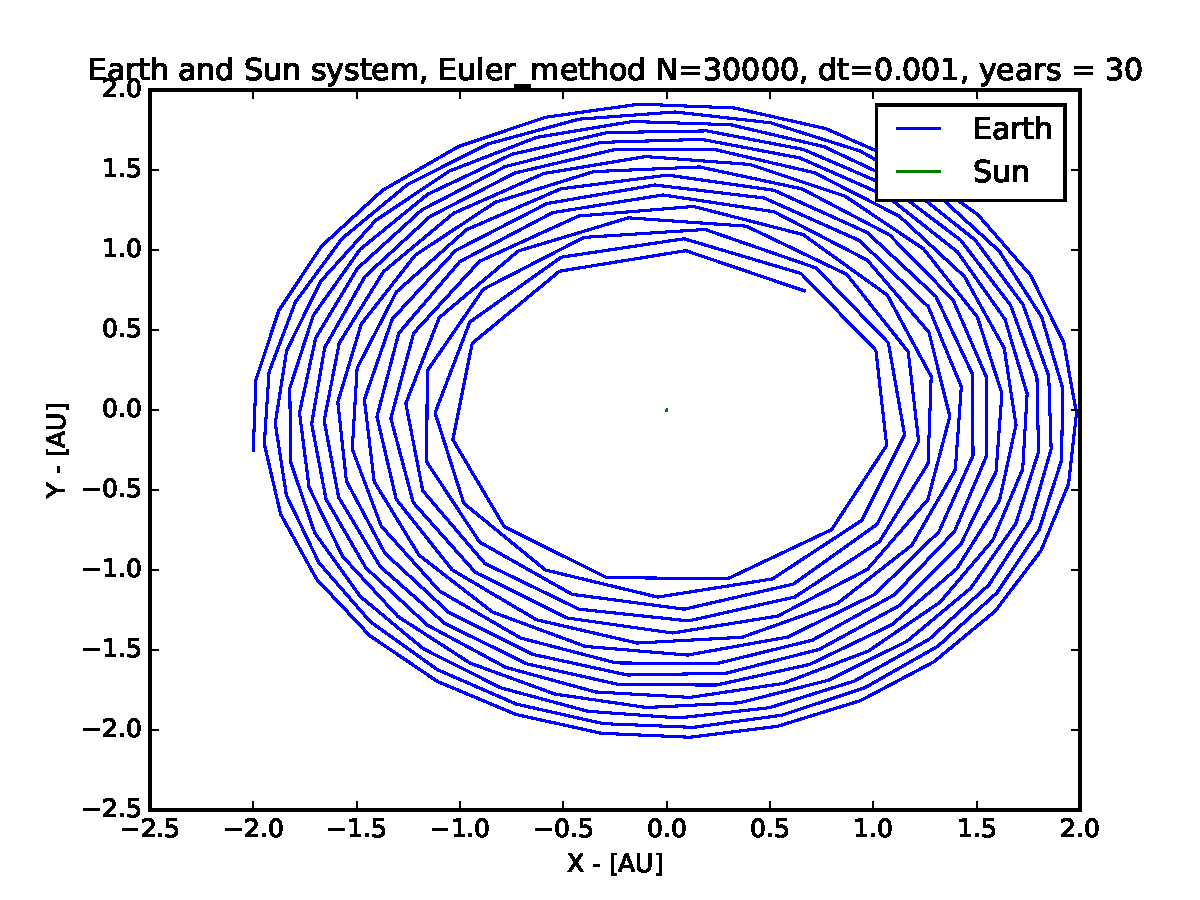
\includegraphics[width=\linewidth]{Plots/Earth_Sun_Euler_method.pdf}
\caption{Euler method using $\Delta t = 10^{-4}$}
\label{fig:balle}
\end{figure}
\begin{figure}[!h]
\centering
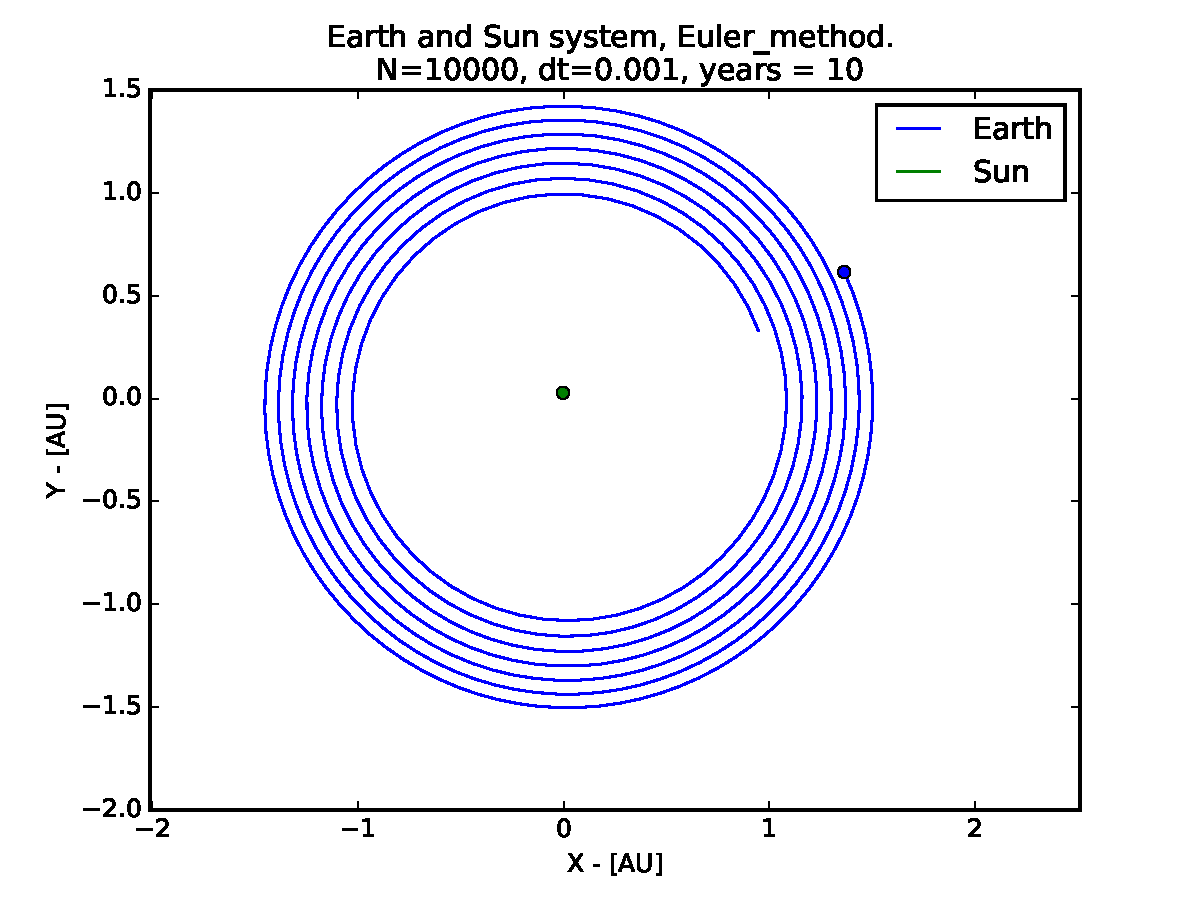
\includegraphics[width=\linewidth]{Plots/Earth_Sun_Euler_method_larger_dt.pdf}
\caption{Euler method using $\Delta t = 10^{-3}$.}
\label{fig:balle1}
\end{figure}
Let us now look at the Verlet method. Figure \ref{fig:balle2} shows the Verlet method using $\Delta t = 10^{-4}$. From this figure, we already see that the Verlet method gives a much better result compared to the ones using the Euler method. Increasing the step length to $\Delta t = 10^{-3}$ would give identical results, so for the Earth-Sun system, Verlet method is very stable up to $\Delta t = 10^{-3}$. A plot for the Verlet method with $\Delta t = 10^{-3}$ can be found in the appendix in figure \ref{fig:balle3}. \\
\begin{figure}[!h]
\centering
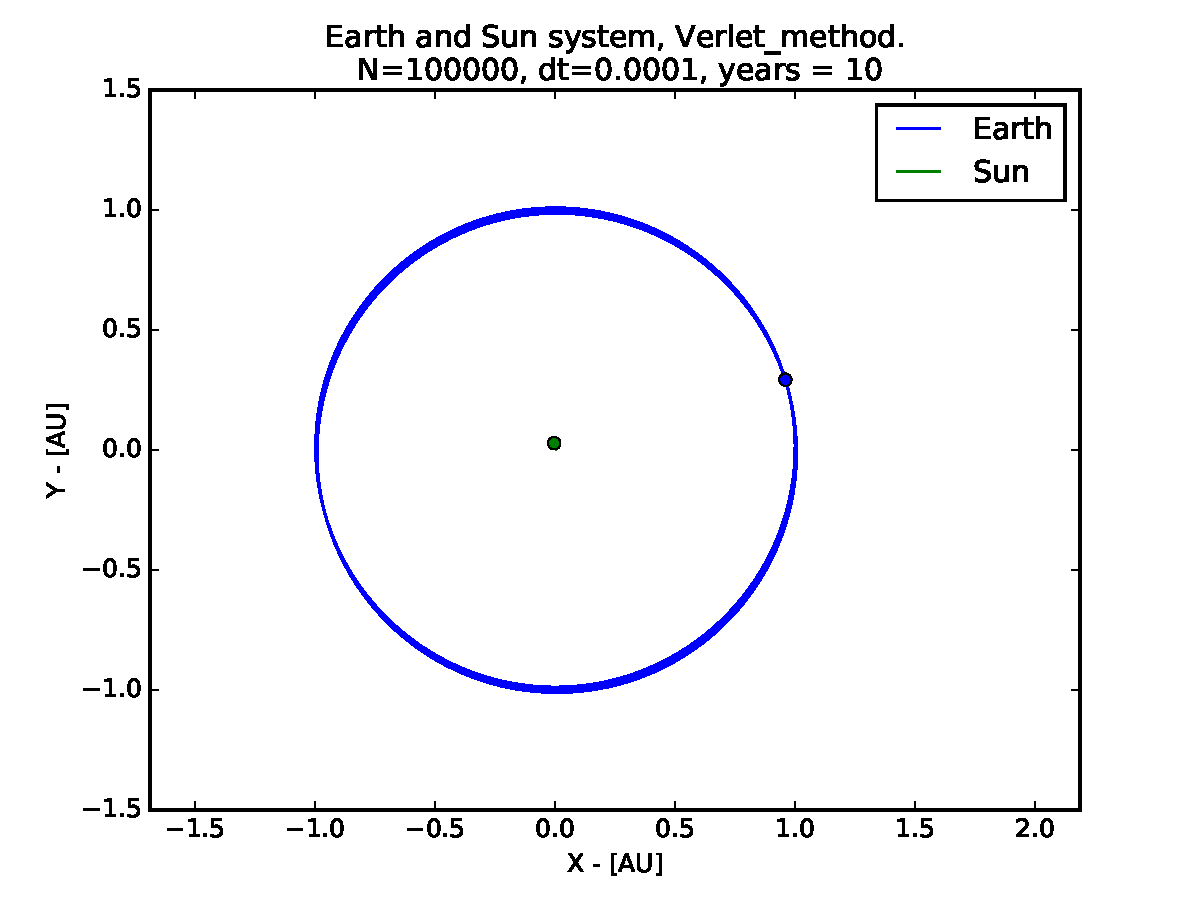
\includegraphics[width=\linewidth]{Plots/Earth_Sun_Verlet_method.pdf}
\caption{Verlet method using $\Delta t = 10^{-4}$}
\label{fig:balle2}
\end{figure}
For the C++ program, the time difference between these two methods are almost negligible for a small number of time steps. As seen in the blue text below, the Verlet method had to run roughly 2 times longer compared to the Euler method, which is not surprising due to the increased number of FLOPS required to solve one time step. However, as we saw from the plots, the extra time it took for the Verlet method gave a much better result than the one using Euler method. Also, as mentioned earlier in the methods sections, when we increase the number of planets we calculate, the computation time between Euler and Verlet method will be negligible. We will therefore stick with the Verlet method for the remainder of the project. \\\\
\begin{lstlisting}
@Running Euler method
Time elapsed for Euler method:0.1s
Data saved to: Earth_Sun_sys_euler.txt

Running Euler Cromer method
Time elapsed for Euler Cromer method:0.097s
Data saved to: Earth_Sun_sys_eulercromer.txt

Running Verlet method
Time elapsed for Verlet method:0.202s
Data saved to: Earth_Sun_sys_verlet.txt@
\end{lstlisting}
Both the total energy and total angular momentum are conserved for the given tolerance, $\epsilon = 3\cdot 10^{-4}$, for all three algorithms, as the output gave no warnings of them. \\\\
One can also use the Euler Cromer method to solve these systems. Figure \ref{fig:Appendix_EulerCromer} shows a plot of the Earth-Sun system using the Euler Cromer method. As we can see, the results practically identical to the Verlet method. The computation speed of the Euler Cromer method is almost identical as the computation speed of the Euler method.

\FloatBarrier
\subsection{Escape velocity}
One can calculate the escape velocity of a planet analytically. The escape velocity of an object with mass $M_1$ is the velocity when the object's kinetic energy is equal to the potential energy. That is
\begin{align*}
\frac{1}{2}M_1v = \frac{GM_1M_2}{r}
\end{align*}
Let us consider a planet with mass $M$ orbiting around the Sun. The escape velocity for this planet is then
\begin{align*}
v_{escape} = \sqrt{\frac{2GM_{\odot}}{r}}
\end{align*}
In terms of AU per year, we have that $GM_{\odot} = 4\pi^2 \text{AU}^3/\text{yr}^2$, so
\begin{align*}
v_{escape} = \sqrt{\frac{8\pi^2}{r}} \text{AU}/\text{yr}
\end{align*}
It is now quite easy to implement the escape velocity. In the C++ program, we have assumed, for simplicity, that the planet has the mass of Earth and start 1 AU away from the Sun in the x direction. The velocity will be the escape velocity directed in the y-direction. \\\\
Figure \ref{fig:EscapeVel} shows a plot of a the planet with mass $M_{earth}$ and how the orbit is if the initial velocity is equal to the escape velocity. As we can see, starting with the escape velocity allows the planet to break free from it's intended orbit and leave the system. The orbit of Earth, with circular orbit used previously, is also plotted as a comparison. \\
\begin{figure}[!h]
\centering
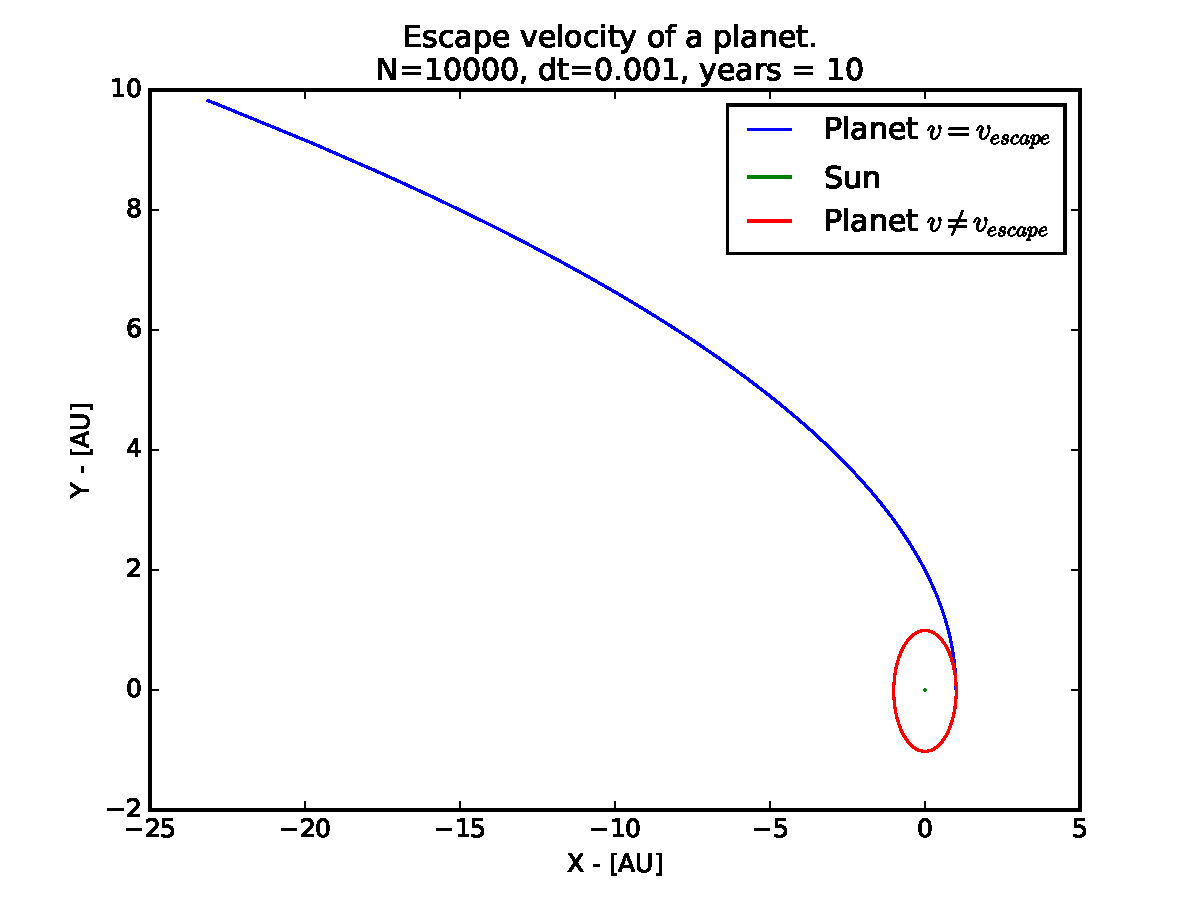
\includegraphics[width=\linewidth]{Plots/Escape_velocity.pdf}
\caption{Plot shows a planet with the mass of Earth with and without escape velocity.}
\label{fig:EscapeVel}
\end{figure}

\FloatBarrier
\subsection{The three-body problem}
From now on, all the initial conditions, i.e positions and velocities of both the Sun and Earth will be obtained from NASA. The date of the data is 2016.10.05. We already know that Earth's orbit will change, from the theory we previously introduced, when we add Jupiter to the system. Figure \ref{fig:EJS_2D_Orbit} shows the orbit of the Earth and Jupiter, as well as the Sun. The orbits themselves does not look particularly odd in any way, but it is hard to see how Jupiter affects the orbit of the Earth. Instead, we only plot the orbit of the Earth and the Sun (still taking Jupiter into account during the calculations) which can be found in figure \ref{fig:EJS_Earth_and_sun}. \\
\begin{figure}[!h]
\centering
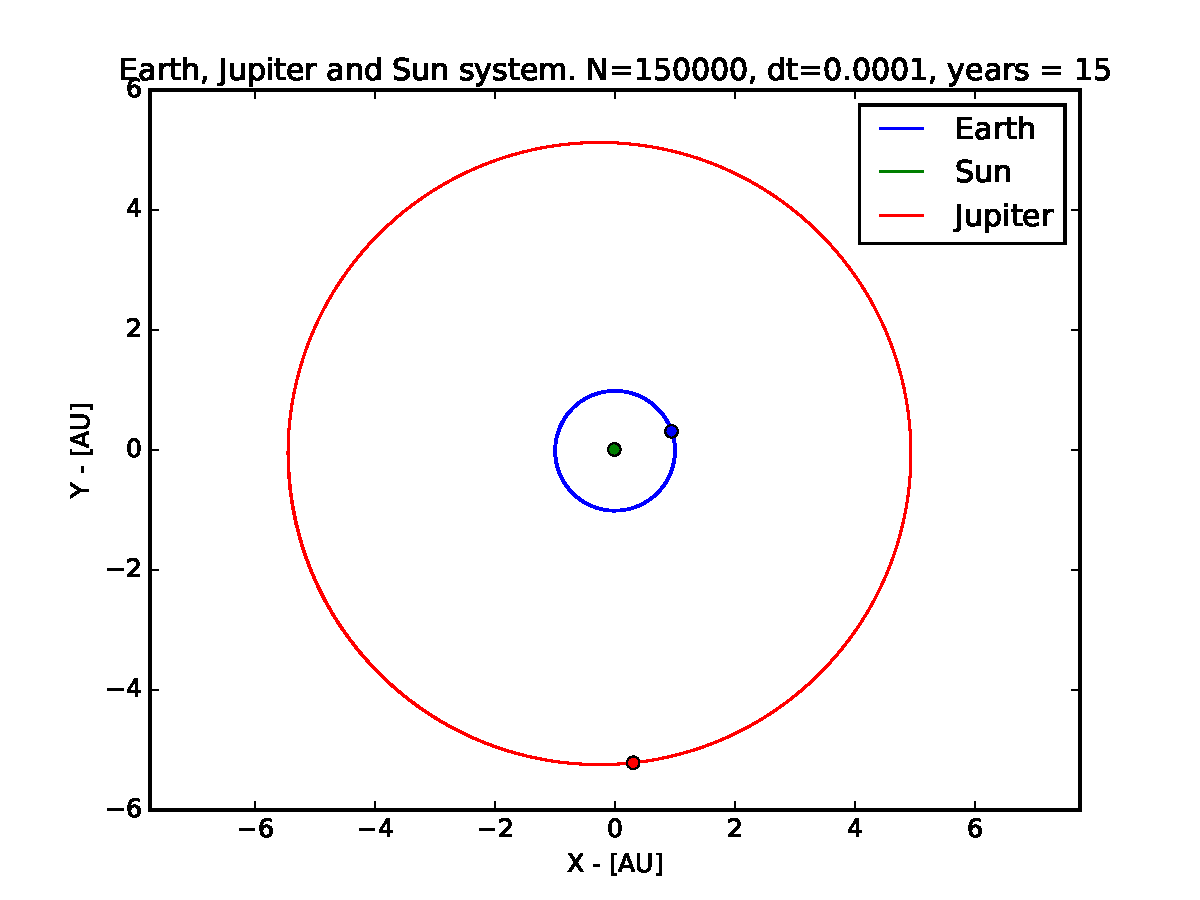
\includegraphics[width=\linewidth]{Plots/Earth_Sun_Jupiter.pdf}
\caption{Orbits of the Earth, Jupiter and the Sun.}
\label{fig:EJS_2D_Orbit}
\end{figure}
\begin{figure}[!h]
\centering
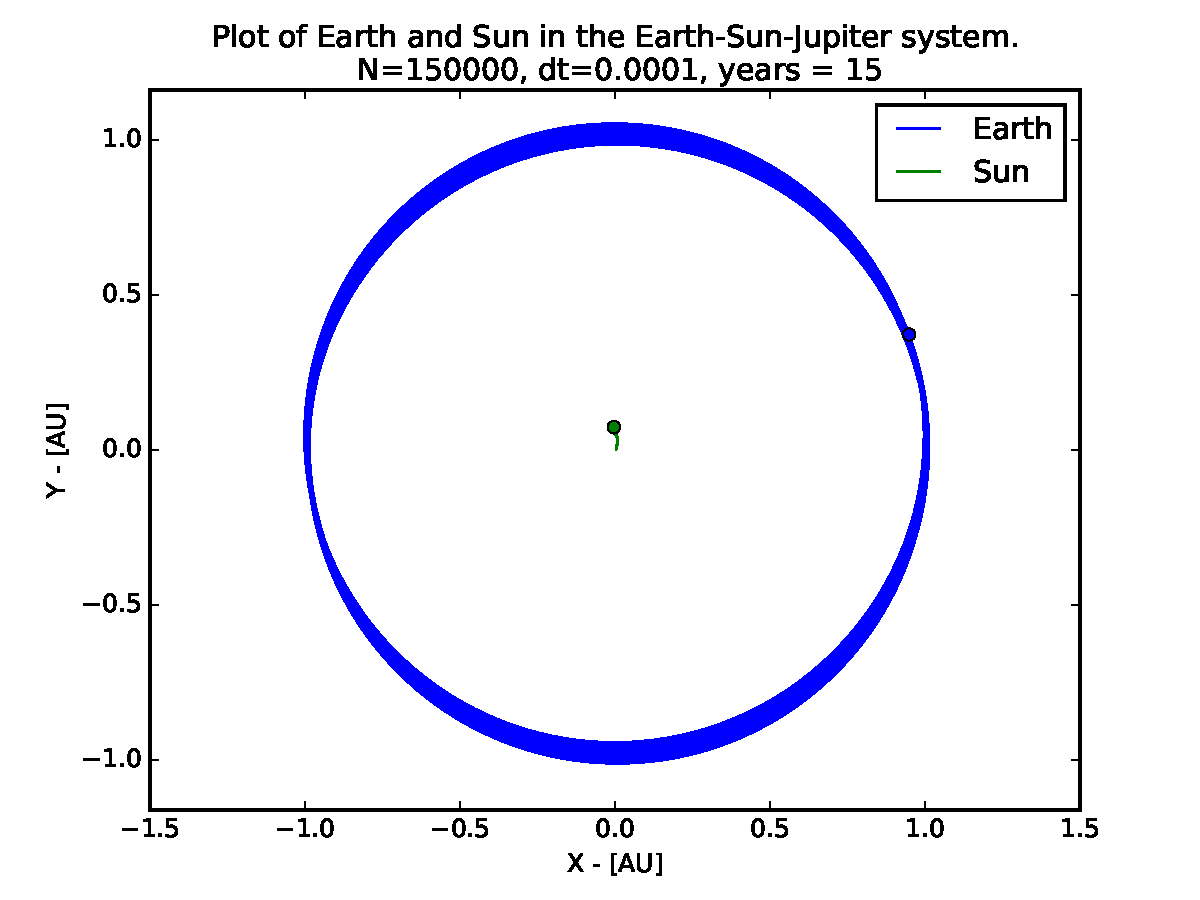
\includegraphics[width=\linewidth]{Plots/ESJ_EarthandSun.pdf}
\caption{Plot of the Earth and the Sun in the Earth-Sun-Jupiter system.}
\label{fig:EJS_Earth_and_sun}
\end{figure}
As we can see from figure \ref{fig:EJS_Earth_and_sun}, the curves tracing the orbits of Earth have changed slightly with respect to each other, since the line appears to be a bit thicker. This indicates that the orbit has become slightly more elliptical. \\\\
The Verlet method for this system is still quite stable, given that $\Delta t = 10^{-4}$. We can also test the stability of the algorithm by increasing the time step to $\Delta t = 10^{-3}$. At the same time, we will have to reduce the number of steps $N$ to match the simulation time. As seen in figure \ref{fig:ESJ_stability} in the appendix, the result is practically identical to the one with $\Delta t = 10^{-4}$. \\\\
Increasing the mass of Jupiter will change the orbits of Earth, the Sun, as well as Jupiter itself even more. Figure \ref{ESJ_10MJ} shows the system when we increase the mass of Jupiter by a factor of 10. We can already see that Earth's orbit has changed a little bit, but the effect of a 10 times more massive Jupiter is not very significant to the whole system. Both planets, even after 20 years, are still in orbit around the Sun. \\
\begin{figure}[!h]
\centering
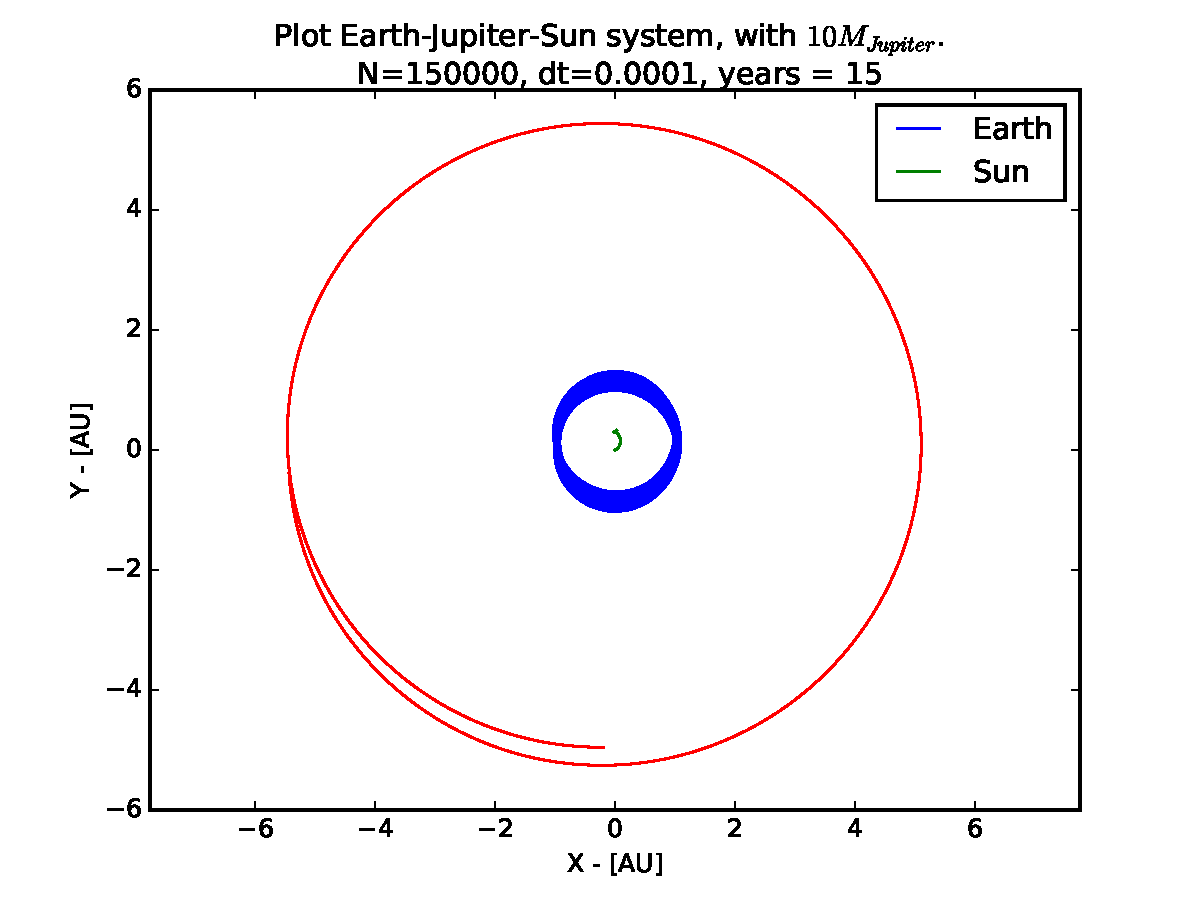
\includegraphics[width=\linewidth]{Plots/Earth_Sun_Jupiter_10MJ.pdf}
\caption{Earth-Sun-Jupiter system for $10M_J$.}
\label{ESJ_10MJ}
\end{figure}
Figure \ref{fig:ESJ_1000MJ} shows the system when the mass of Jupiter is increased by a factor of $1000$, and the result is very interesting. At this point, Jupiter has practically the same mass the Sun, so the gravitational effects from that should be quite dramatic. As we see from the figure, the Sun starts to move due to the increased mass of Jupiter. We also notice that Earth is getting flung around between these two massive objects. \\\\
The center of mass (CM) also starts to move because of the increased mass of Jupiter. The movement of the CM depends on the momentum of each object. Now that Jupiter has an increased mass, and the initial velocity is unchanged, the sudden increase of momentum will shift the CM as a whole. \\\\
3D Plots of this system with unchanged Jupiter mass and $1000$ times the Jupiter mass can be found in the appendix in figure \ref{fig:Appendix_3D_ESJ} and \ref{fig:Appendix_1000MJ} respectively. \\
\begin{figure}[!h]
\centering
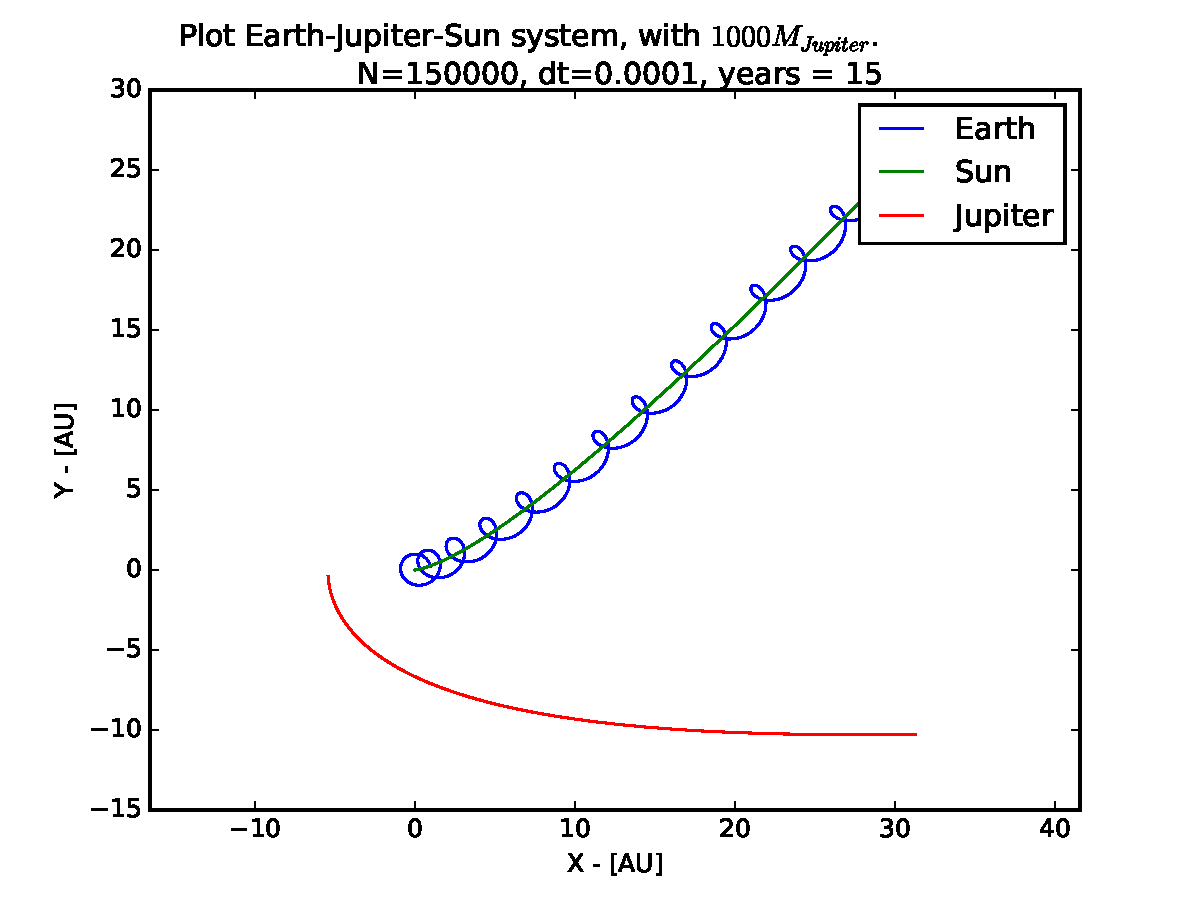
\includegraphics[width=\linewidth]{Plots/Earth_Sun_Jupiter_1000MJ.pdf}
\caption{Earth-Sun-Jupiter system for $1000M_J$.}
\label{fig:ESJ_1000MJ}
\end{figure}

\FloatBarrier
\subsection{All planets}
We will now add all planets, including Pluto, into our system. This is quite straight forward to do. In the C++ program, all we have to do is to add an extra force to each planet. Figure \ref{fig:All_planets_3D} shows the orbits of all planets in 3 dimensions, for 250 years. The initial velocity of the Sun is set, so that the total momentum of the system is conserved, that is
\begin{align}
M_{\odot}v_{\odot} + \displaystyle \sum_i M_i v_i = 0
\end{align}
\begin{figure}[!h]
\centering
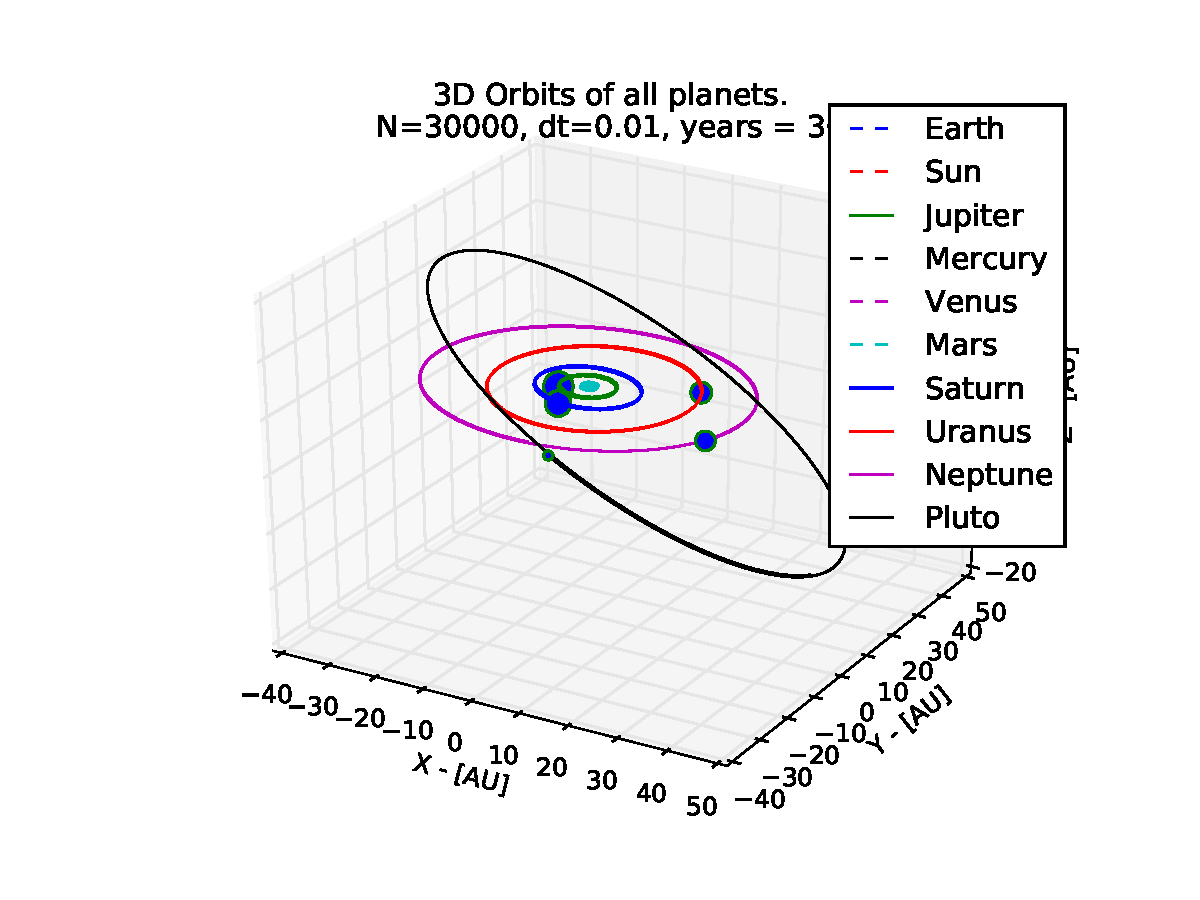
\includegraphics[width=\linewidth]{Plots/All_planets_3D_plot.pdf}
\caption{Plot of all planets in 3D. Note: the scatter plot (spheres) of the planet does not scale with it's real size.}
\label{fig:All_planets_3D}
\end{figure}
Because of the orbit sizes of the outer planets (i.e Jupiter, Saturn, Uranus, Neptune and Pluto), the orbits of the first four planets will be packed in the center of the system, which is quite hard to analyse. What we can do is to only plot the first four planets, while still taking the effect of the gravitational effects of the other planets into account. \\\\
However, plotting 250 years worth of orbits of the first four planets are quite redundant so we have decided to reduce the number of time steps, $\Delta t$. This is to, again, mainly to reduce the number of simulated years, but it will also increase the stability of the Verlet method. The orbits of the first four planets under these settings can be found in figure \ref{fig:First4_planets_3D}. One thing to note is that the outer planets will no longer have full orbits, like in figure \ref{fig:All_planets_3D}. However, the effect from the gravitational pull of these planets are still present, which is the most important part. \\
\begin{figure}[!h]
\centering
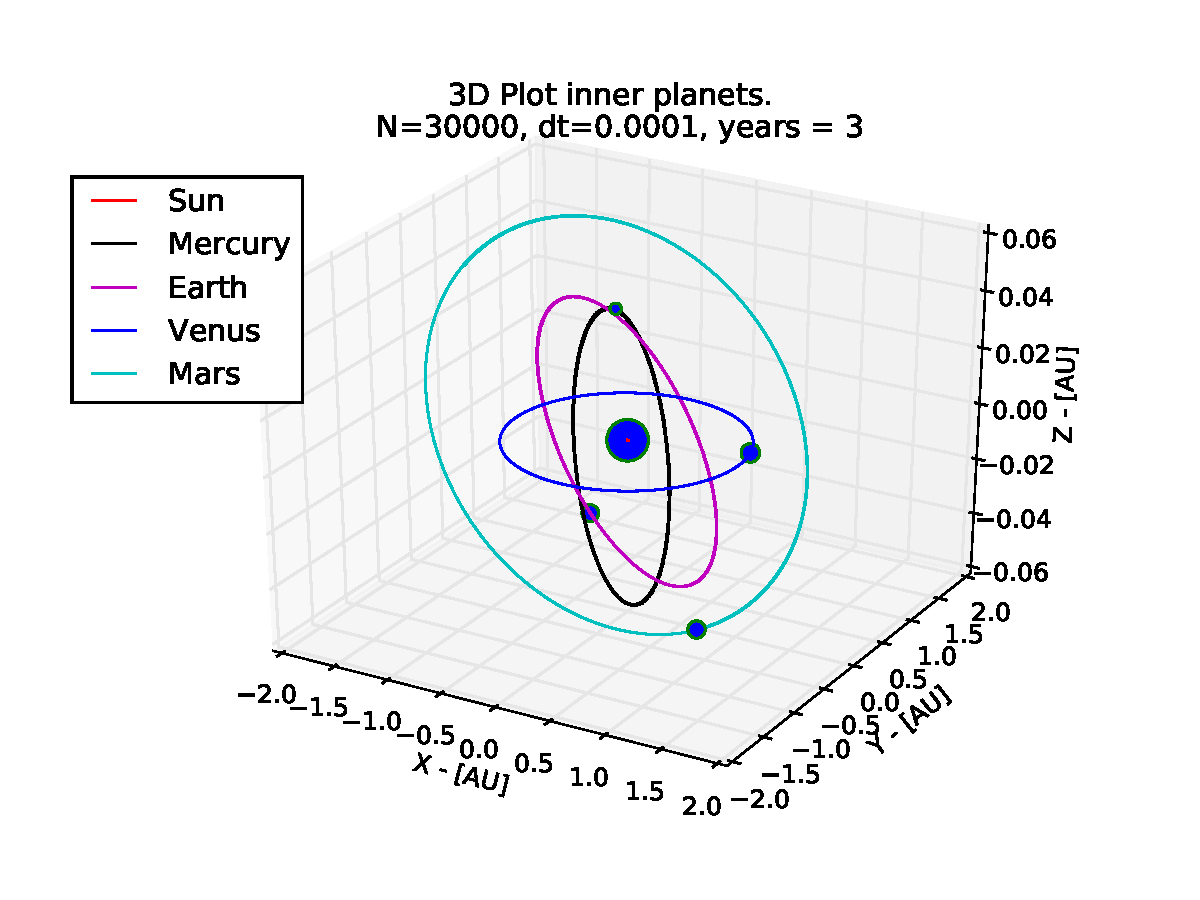
\includegraphics[width=\linewidth]{Plots/First_planets_3D_plot.pdf}
\caption{3D plot of the first four planets orbit. Note: the scatter plot (spheres) of the planet does not scale with it's real size.}
\label{fig:First4_planets_3D}
\end{figure}
The results are promising. The orbits of all planets resembles the orbits we observe. When looking at the plot for the first four planets, one may quickly be confused by the orbits, as it seems like the planets (with the exception of Earth) goes very high up in the z-axis. But this movement is at most up to $\pm 0.04AU$, which is a very small movement. By looking at figure \ref{fig:All_planets_3D}, the vertical movement of the first four planets are practically zero, when we include Pluto to the system.

\FloatBarrier
\subsection{Precession of Mercury's perihelion} \label{section:mprec}
In this section we discuss our simulation of Mercury's perihelion precession due to general relativity, which uses the correction to Newtonian gravitation described in section \ref{section:gcorr}. There are several effects that cause the orientation of Mercury's orbit to change over time, the most important of which being the gravitational forces from the other planets. When trying to reproduce the much smaller precession caused by general relativity, we therefore limited ourselves to the two-body system of the sun and Mercury. \\\\
We initialised a simulation with the center of mass at the origin, and Mercury in the perihelion position $\mb{r}_{21} = (0.3075, 0, 0)$ with the perihelion velocity $\mb{v}_{21} = (0, 12.44, 0)$ (note that the units are still AU for length and years for time). The sun was given a corresponding speed in the opposite direction in order to make the center of mass stationary. \\\\
A high degree of precision was required to resolve the minute variations in the perihelion position. As mention in section \ref{section:gcorr}, the orientation of the orbit changes by about $43''$, or $2.08\cdot 10^{-4}\;\text{rad}$, per century. At perihelion this corresponds to a physical distance of $0.3075\;\text{AU}\cdot 2.08\cdot 10^{-4}\;\text{rad} = 6.4\cdot 10^{-5}\;\text{AU} = 9570\;\text{km}$. Mercury traverses this distance in $6.4\cdot 10^{-5}\;\text{AU}/12.44\;\text{AU}\;\text{yr}^{-1} = 5.14\cdot 10^{-6}\;\text{yr} = 162\;\text{s}$. How finely we resolve Mercury's movement will decide the precision to which we can determine the precession angle. If the angular distance between two subsequent positions near the perihelion is $\Delta \theta$, our measurement of the perihelion angle should have a precision of $\pm \Delta \theta/2$. If we require $\Delta \theta = 1''$, we need a distance of $0.3075\;\text{AU}\cdot 1'' = 0.3075\;\text{AU}\cdot 4.85\cdot 10^{-6}\;\text{rad} = 1.49\cdot 10^{-6}\;\text{AU}$, or about 223 km, between each measurement. The required temporal resolution for this is $1.49\cdot 10^{-6}\;\text{AU}/12.44\;\text{AU}\;\text{yr}^{-1} = 1.20\cdot 10^{-7}\;\text{yr}$, which is just below 4 seconds. If we use a constant time step size, this corresponds to over 800 million time steps for a 100 year simulation. To avoid having to handle such a large amount of output data, we adjusted the code to let us write the results to file only for the final orbit, since this is all we need to measure the final perihelion position. \\\\
Figure \ref{fig:pprec} is a plot of a section of the first and last orbit of a 100 year simulation, with the perihelion positions of the orbits indicated. \\
\begin{figure}[!h]
    \centering
    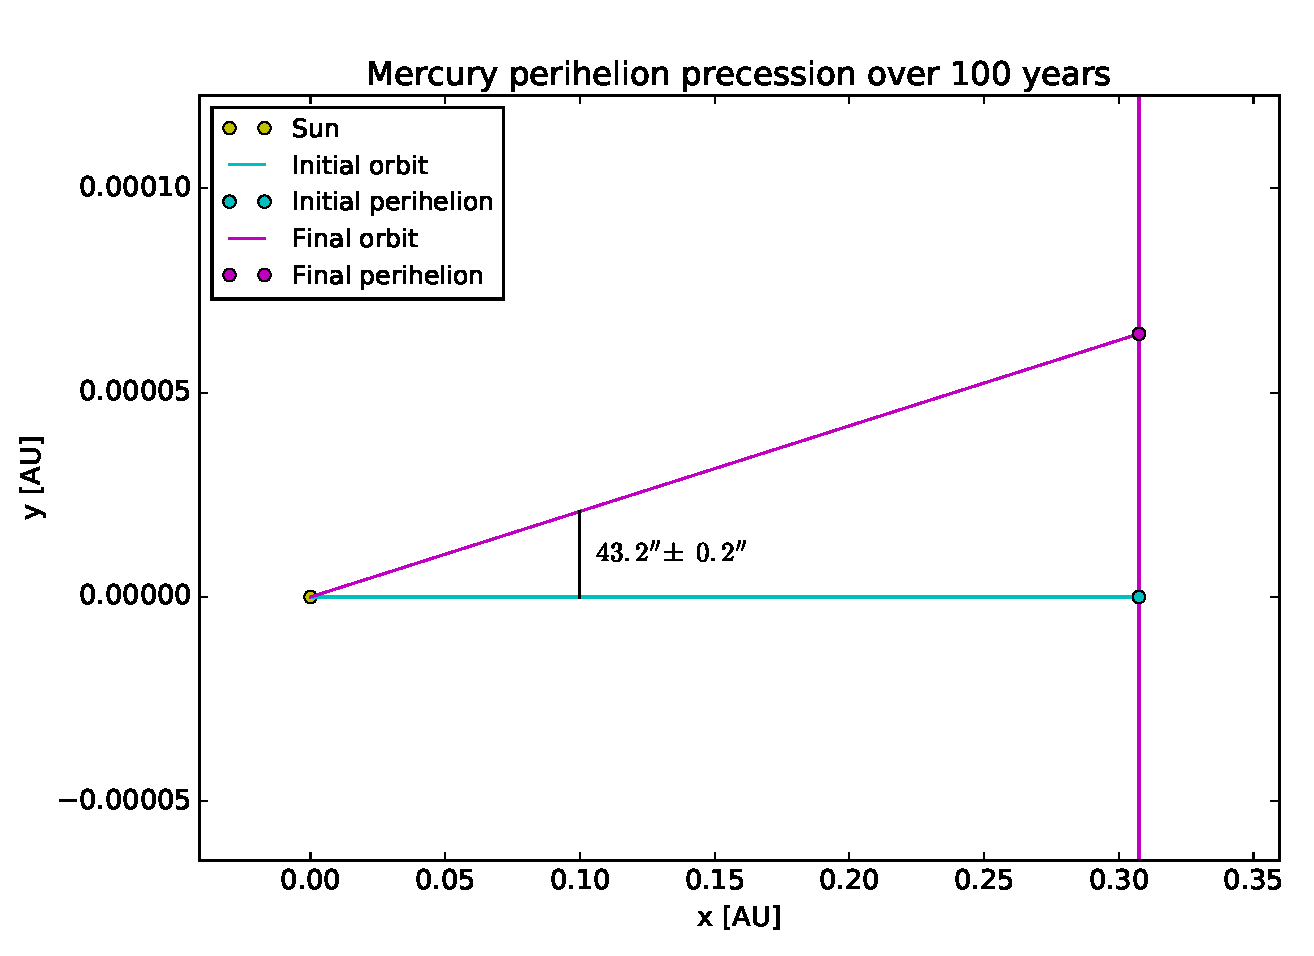
\includegraphics[width=\linewidth]{perihelion_precession.pdf}
    \caption{Plot of two orbits of Mercury separated by 100 years. Note that the plot is strongly zoomed in the $y$-direction to show the minute difference between the two perihelions, causing the orbits to appear to overlap completely.}
    \label{fig:pprec}
\end{figure}\\
The angle between the two lines connecting the sun and the perihelions is the precession angle. The time step size used for this simulation was about $6\cdot 10^{-8}\;\text{yr}$, giving a precision of about $\pm 0.2''$. We see that our result of $43.2''$ agrees with the observed precession angle. Figure \ref{fig:pprec2} gives a closer view to better show the difference between the two orbits. \\
\begin{figure}[!h]
    \centering
    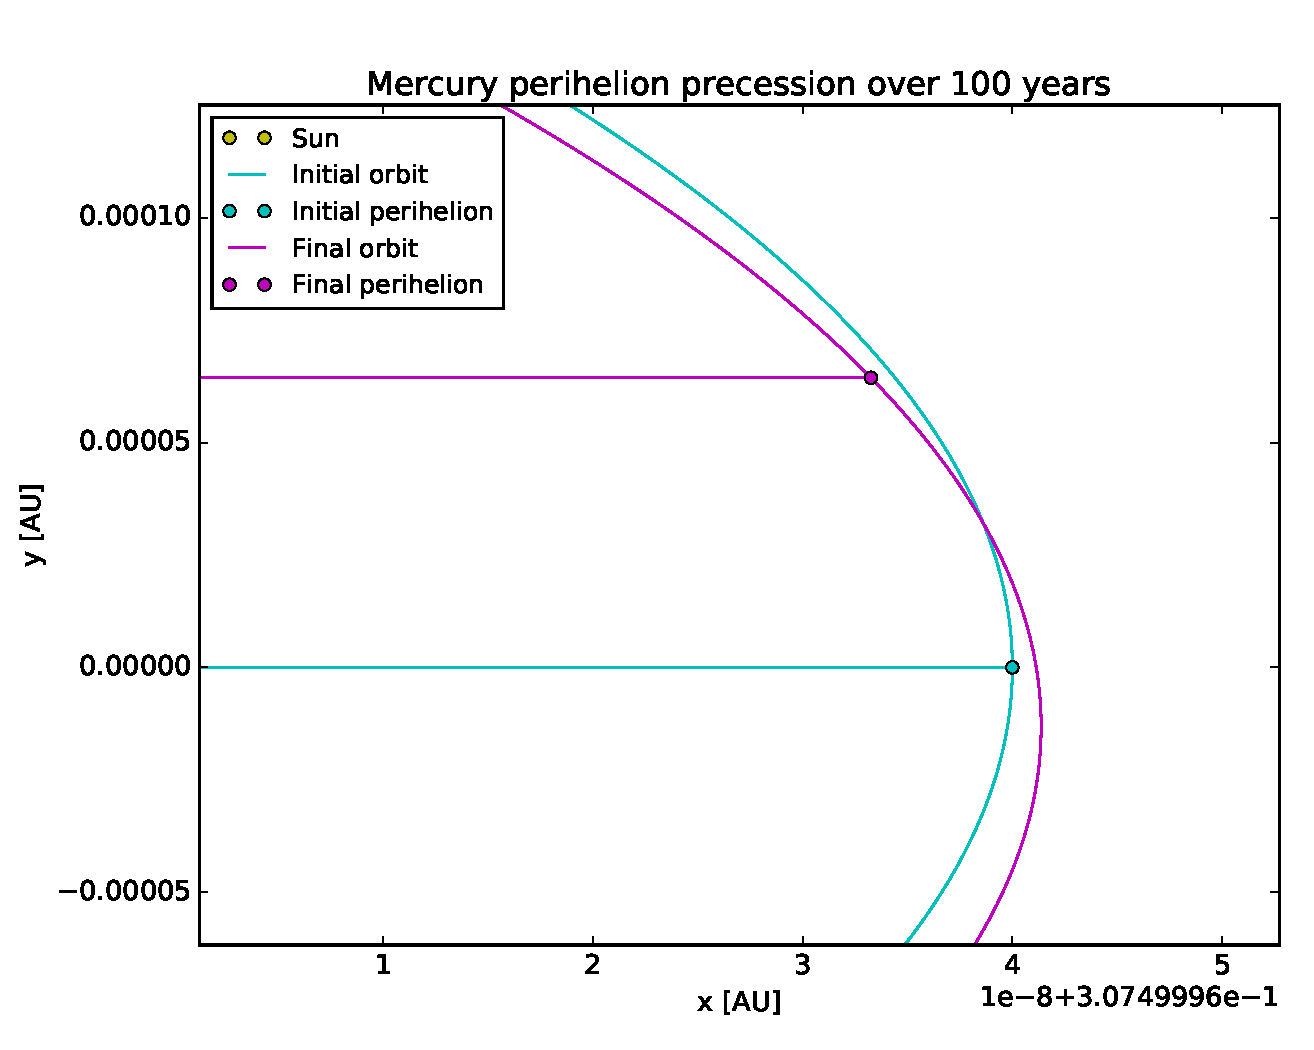
\includegraphics[width=\linewidth]{perihelion_precession_2.pdf}
    \caption{The same orbits as in figure \ref{fig:pprec} are here shown with a very strong zoom in the $x$-direction to make the different orientations of the orbits visible.}
    \label{fig:pprec2}
\end{figure}

\FloatBarrier
\section{Conclusions} \label{section:conc}
As we saw when we simulated the Earth-Sun system, the Verlet method was clearly the algorithm of choice, as the Euler method did not give stable circular systems. Even though the Verlet method requires more FLOPS to run, the computation time between it and the Euler method is negligible when we start to add more objects to the system. \\\\
All the planetary orbits, whether it was for Earth-Sun system, Earth-Sun-Jupiter system or even the whole Solar system, gave promising results that resembles real orbits we observe. Increasing the mass of one of the Planets, as seen in the three body problem, changed the orbits of all the celestial objects. If we increase the mass enough, then the system would be very chaotic, which we saw when we increased Jupiter's mass by 1000. \\\\
With the general relativistic correction we were also able to reproduce the observed precession of Mercury's orbit.

\section{Appendix}
\begin{figure}[!h]
\centering
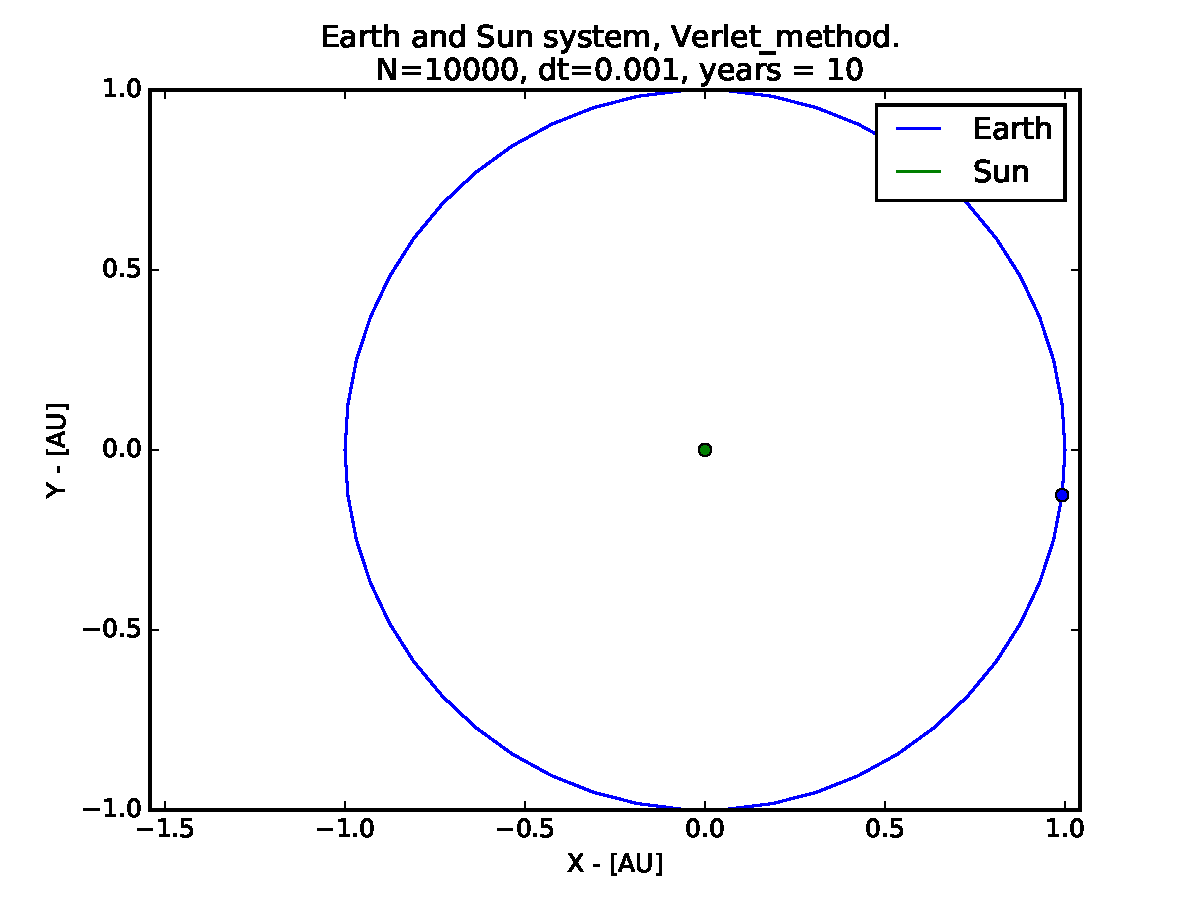
\includegraphics[width=\linewidth]{Plots/Earth_Sun_Verlet_method_larger_dt.pdf}
\caption{Verlet method using $\Delta t = 10^{-3}$}
\label{fig:balle3}
\end{figure}
\begin{figure}[!h]
\centering
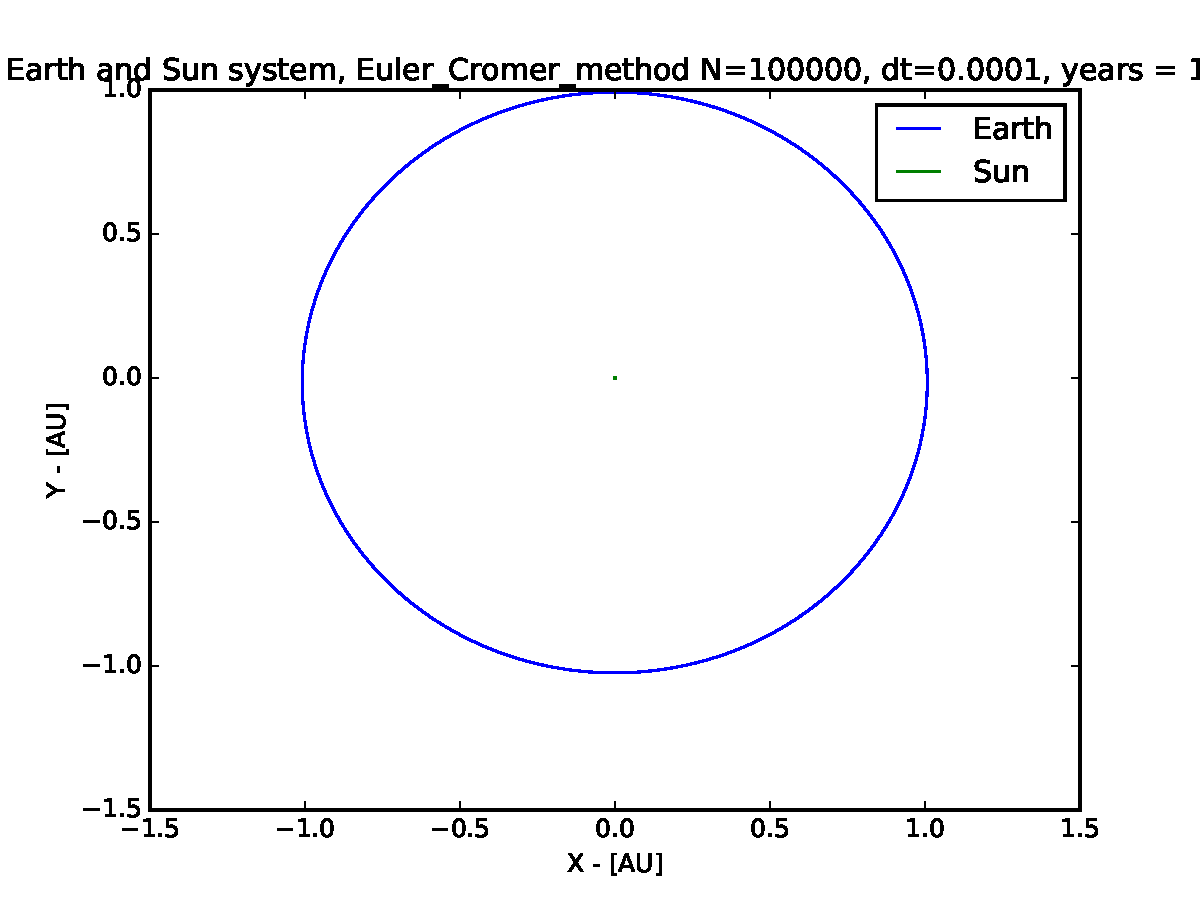
\includegraphics[width=\linewidth]{Plots/Earth_Sun_Euler_Cromer_method.pdf}
\caption{Earth-Sun system using Euler Cromer method}
\label{fig:Appendix_EulerCromer}
\end{figure}
\begin{figure}[!h]
\centering
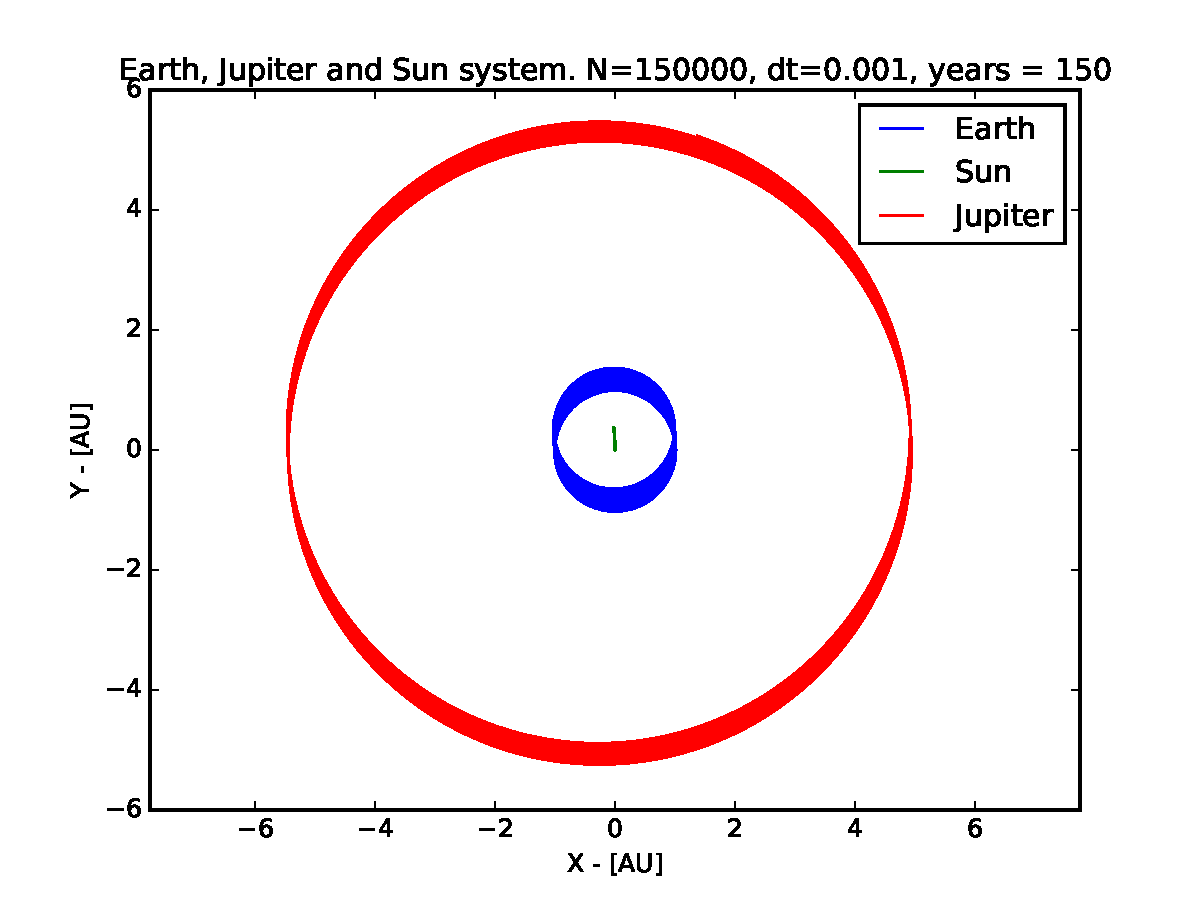
\includegraphics[width=\linewidth]{Plots/Earth_Sun_Jupiter_largerdt.pdf}
\caption{Earth-Sun-Jupiter system for $\Delta t = 10^{-3}$. The result is identical to the system with $\Delta t = 10^{-4}$.}
\label{fig:ESJ_stability}
\end{figure}
\begin{figure}[!h]
\centering
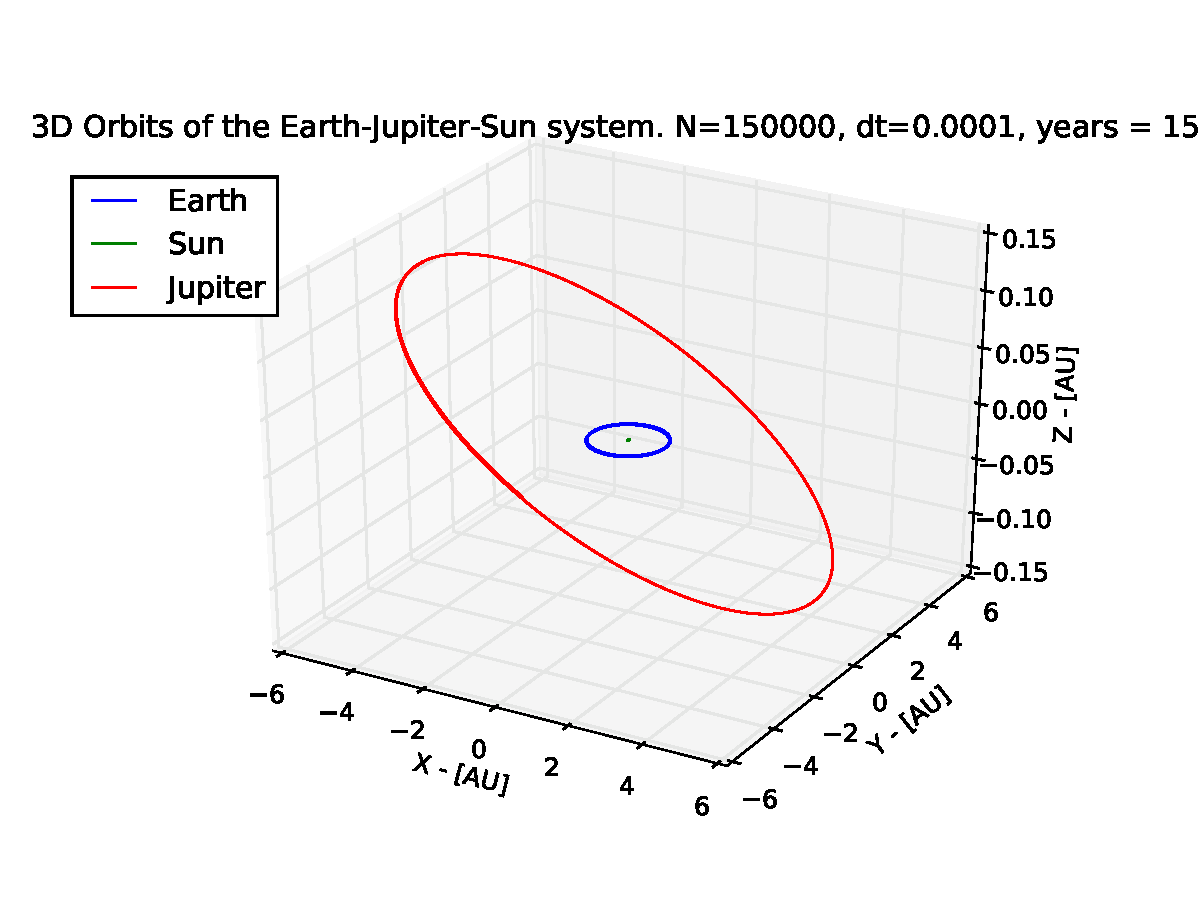
\includegraphics[width=\linewidth]{Plots/Earth_Sun_Jupiter_3D.pdf}
\caption{3D Plot of the Earth-Sun-Jupiter system.}
\label{fig:Appendix_3D_ESJ}
\end{figure}
\begin{figure}[!h]
\centering
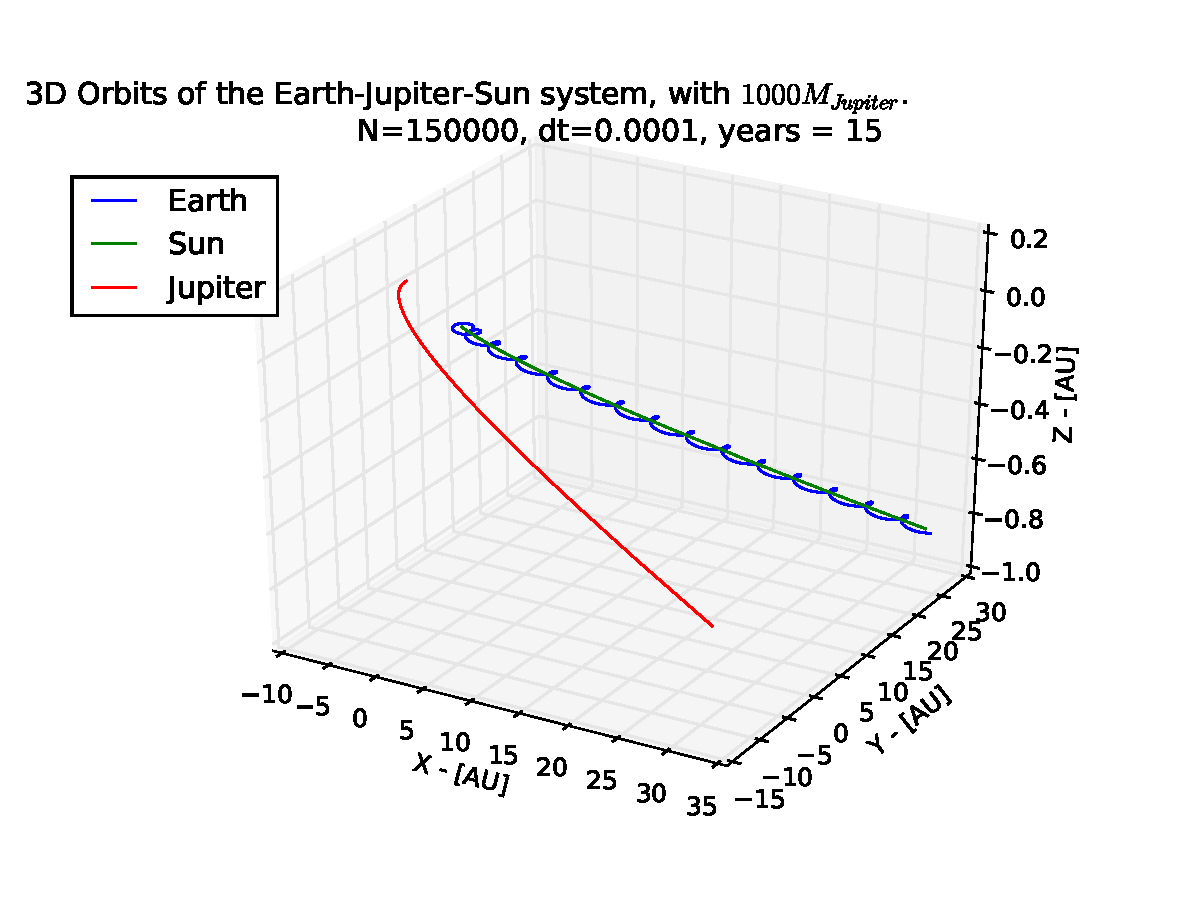
\includegraphics[width=\linewidth]{Plots/Earth_Sun_Jupiter_1000MJ_3D.pdf}
\caption{3D plot for Earth-Sun-Jupiter system with the mass of Jupiter as $1000M_{Jupiter}$}
\label{fig:Appendix_1000MJ}
\end{figure}

\FloatBarrier
\begin{thebibliography}{1}
    \bibitem{cpyhsics} M. Hjorth-Jensen, \emph{Computational Physics}, 2015, 551 pages
\end{thebibliography}

\end{document}
